

\subsection{as\_picam}

\secauthor{Thomas Izycki}

The \texttt{as\_picam} module was developed in order to use a \textit{Raspberry Pi} camera v1.3 or v2.1 with an \asterics chain on a TE0726 Zynqberry\footnote{\url{https://shop.trenz-electronic.de/en/TE0726-03M-ZynqBerry-Module-with-Xilinx-Zynq-7010-in-Raspberry-Pi-Form-Faktor}}. It is operated in combination with the \texttt{video\_in} subsystem provided by \textit{Trenz Electronic GmbH}. The subsystem consists of several modules and interfaces the camera by implementing the CSI-2 specification. As long as the \textit{enable} signal is active, a continuous video stream is apllied to its AXI-Stream output with 8-bit per pixel in the ABGR format.
For further information on the \texttt{video\_in} subsystem refer to section \ref{sec:09-01-as_refdesign_zynqberry}.

\subsubsection{Module Description}

The \texttt{as\_picam} module serves as a link between the \texttt{video\_in} subsystem and the \asterics chain with image data being transmitted via AXI-Stream. A constant enable signal applied to the \texttt{video\_in} subsystem keeps the camera permanently in operation, generating a steady video stream. In addition the AXI-Stream's \textit{READY} signal is also kept high the entire time, meaning new data is accepted every clock cycle. For use within the ASTERICS chain the \texttt{as\_picam} module provides an \texttt{as\_stream} output interface. Figure \ref{07-as-picam-wave} shows the AXI-Stream input compared to the \texttt{as\_stream} output at the beginning of a new image frame, indicated by the \textit{start of frame} (SOF) signal.

\begin{figure}[htbp]
    \noindent \begin{centering}
    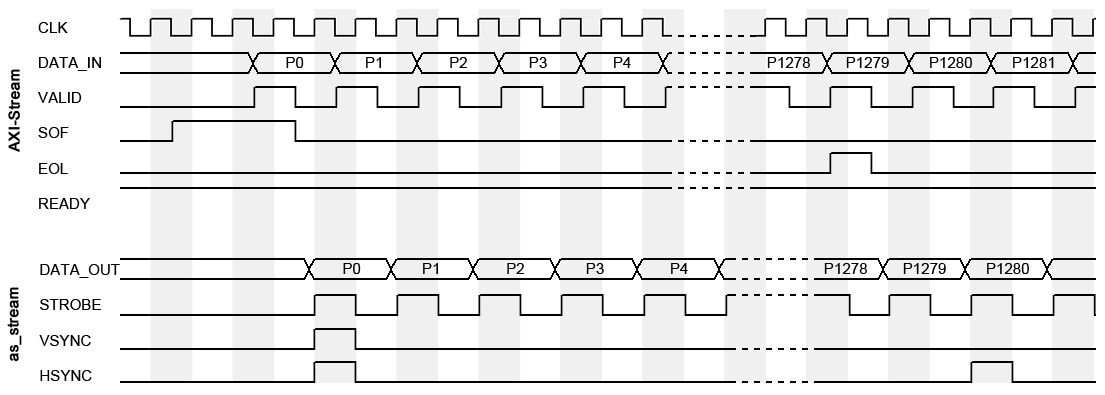
\includegraphics[width=\textwidth]{figs/07-as_picam_wave.png}
    \par\end{centering}
    \caption{Conversion of AXI-Stream to as\_stream}
    \label{07-as-picam-wave}
\end{figure}

In contrast to the \texttt{as\_stream} specification that needs the \textit{HSYNC} signal to be generated with the first pixel of every line, the AXI-Stream protocol defines the \textit{end of line} (EOL) signal occurring with the last pixel of a line.
Beside the AXI-Stream to \texttt{as\_stream} conversion the 32-bit BGRA image data is transformed into 8-bit grayscale.
\subsubsection{Register Space}

The module has one 32-bit wide combined status and control register depicted in Table \ref{07-as-picam-register}.

\begin{longtable}[htb]{|c|c|c|c|}
\hline
\textbf{Bit Name} & \textbf{Index} & \textbf{Access} & \textbf{Description} \\
\hline
\endhead

\texttt{Frame Done} & 0 & R &
\parbox{8,5cm}{ ~ \\ Frame completely transmitted. \\ ~  \small
This status bit is set by the hardware when the last pixel of an image has been transferred.
\vspace{0.3em} ~ } \\

\hline

\texttt{Data Enable} & 17 & W &
\parbox{8,5cm}{ ~ \\ Enables the video stream. \\ ~ \small
As soon as this bit is set, the camera images are output continously as grayscale images.
\vspace{0.3em} ~ } \\

\hline

\texttt{Enable Once} & 18 & W &
\parbox{8,5cm}{ ~ \\ Process one image. \\ ~  \small
Setting this bit has the effect that exactly one complete image is output as a grayscale image.
\vspace{0.3em} ~ } \\

\hline

\caption{Bit fields of the status and control register}
\label{07-as-picam-register}
\end{longtable}

\subsubsection{Software Driver}

The software driver serves two purposes. The first one is to initialize the \textit{Raspberry Pi} camera by configuring it via \textit{i2c}. Therefore the processing system's \textit{i2c} module is used and the corresponding setup is loaded into the camera's registers. However, only resolutions of 1280x720 pixels are supported. The distinction between the \textit{Raspberry Pi} camera v1.3 and 2.1 is made automatically.
The second purpose is to interface the hardware. Either the camera is set to a constant run mode, streaming the video data or every frame is triggered individually.
